% Graphic for TeX using PGF
% Title: /home/enberg/Diagram4.dia
% Creator: Dia v0.97.2
% CreationDate: Mon Apr 28 21:29:10 2014
% For: enberg
% \usepackage{tikz}
% The following commands are not supported in PSTricks at present
% We define them conditionally, so when they are implemented,
% this pgf file will use them.
\ifx\du\undefined
  \newlength{\du}
\fi
\setlength{\du}{15\unitlength}
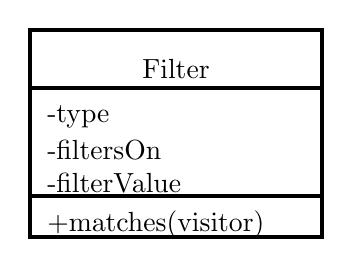
\begin{tikzpicture}
\pgftransformxscale{1.000000}
\pgftransformyscale{-1.000000}
\definecolor{dialinecolor}{rgb}{0.000000, 0.000000, 0.000000}
\pgfsetstrokecolor{dialinecolor}
\definecolor{dialinecolor}{rgb}{1.000000, 1.000000, 1.000000}
\pgfsetfillcolor{dialinecolor}
\pgfsetlinewidth{0.100000\du}
\pgfsetdash{}{0pt}
\definecolor{dialinecolor}{rgb}{1.000000, 1.000000, 1.000000}
\pgfsetfillcolor{dialinecolor}
\fill (17.500000\du,11.450000\du)--(17.500000\du,12.850000\du)--(24.545000\du,12.850000\du)--(24.545000\du,11.450000\du)--cycle;
\definecolor{dialinecolor}{rgb}{0.000000, 0.000000, 0.000000}
\pgfsetstrokecolor{dialinecolor}
\draw (17.500000\du,11.450000\du)--(17.500000\du,12.850000\du)--(24.545000\du,12.850000\du)--(24.545000\du,11.450000\du)--cycle;
% setfont left to latex
\definecolor{dialinecolor}{rgb}{0.000000, 0.000000, 0.000000}
\pgfsetstrokecolor{dialinecolor}
\node at (21.022500\du,12.400000\du){Filter};
\definecolor{dialinecolor}{rgb}{1.000000, 1.000000, 1.000000}
\pgfsetfillcolor{dialinecolor}
\fill (17.500000\du,12.850000\du)--(17.500000\du,15.450000\du)--(24.545000\du,15.450000\du)--(24.545000\du,12.850000\du)--cycle;
\definecolor{dialinecolor}{rgb}{0.000000, 0.000000, 0.000000}
\pgfsetstrokecolor{dialinecolor}
\draw (17.500000\du,12.850000\du)--(17.500000\du,15.450000\du)--(24.545000\du,15.450000\du)--(24.545000\du,12.850000\du)--cycle;
% setfont left to latex
\definecolor{dialinecolor}{rgb}{0.000000, 0.000000, 0.000000}
\pgfsetstrokecolor{dialinecolor}
\node[anchor=west] at (17.650000\du,13.550000\du){-type};
% setfont left to latex
\definecolor{dialinecolor}{rgb}{0.000000, 0.000000, 0.000000}
\pgfsetstrokecolor{dialinecolor}
\node[anchor=west] at (17.650000\du,14.350000\du){-filtersOn};
% setfont left to latex
\definecolor{dialinecolor}{rgb}{0.000000, 0.000000, 0.000000}
\pgfsetstrokecolor{dialinecolor}
\node[anchor=west] at (17.650000\du,15.150000\du){-filterValue};
\definecolor{dialinecolor}{rgb}{1.000000, 1.000000, 1.000000}
\pgfsetfillcolor{dialinecolor}
\fill (17.500000\du,15.450000\du)--(17.500000\du,16.450000\du)--(24.545000\du,16.450000\du)--(24.545000\du,15.450000\du)--cycle;
\definecolor{dialinecolor}{rgb}{0.000000, 0.000000, 0.000000}
\pgfsetstrokecolor{dialinecolor}
\draw (17.500000\du,15.450000\du)--(17.500000\du,16.450000\du)--(24.545000\du,16.450000\du)--(24.545000\du,15.450000\du)--cycle;
% setfont left to latex
\definecolor{dialinecolor}{rgb}{0.000000, 0.000000, 0.000000}
\pgfsetstrokecolor{dialinecolor}
\node[anchor=west] at (17.650000\du,16.150000\du){+matches(visitor)};
\end{tikzpicture}
